\documentclass[10pt,a4paper]{report}
\usepackage[utf8]{inputenc}
\usepackage[francais]{babel}
\usepackage{setspace}
\usepackage[T1]{fontenc}
\usepackage{float}
\usepackage{hyperref}
\usepackage{amsmath}
\usepackage{amsfonts}
\usepackage{amssymb}
\usepackage{graphicx}
\author{Baptiste Lesquoy}
\title{Rapport de projet de synthèse}
\date{25 novembre 2014}
\begin{document}
\begin{spacing}{0.8}

%%%%%%%%%%%%%%%%%%%%%%%% PAGE DE GARDE
\maketitle
\newpage


%%%%%%%%%%%%%%%%%%%%%%% TABLE DES MATIÈRES
\tableofcontents
\newpage

\chapter{Introduction}
Dans le cadre du projet de synthèse de la L3 informatique, il nous a été demandé de réaliser une application client serveur. Cette dernière a pour but de permettre la création et la modification des formes géométriques côté client, puis de les envoyer au serveur pour que celui-ci les dessine.


\chapter{Choix de programmation vis à vis du sujet}

\section{renvoie de copie}
Il a été décidé de ne pas transformer directement les formes par les opérations, mais plutôt un nouvel objet qui correspond à la forme transformée. De cette manière on garde toutes les formes immuables.

\section{vis à l'extérieur d'un groupe}
Comme il fallait faire un choix, la classe \textit{Groupe} ne contient pas de copie des objets mais uniquement les pointeurs sur ces derniers, qui de toute façon sont immuables.
\section{Protocole de communication}\label{protocole}
Le facteur humain n'étant pas demandé, les formats xml et json ont pu être écarté au profit dans format plus simple (mais néanmoins toujours relativement lisible),qui est: "type: couleur, point.." pour les types simple ou "groupe couleur(objet1;objet2 ...)" pour les groupes.

\section{Utilisation de toString()}\label{toString}
La fonction toString renvoie une chaîne correspondant à la représentation de la classe à un moment donnée, mais la chaîne renvoyée est plus que ça, elle suit le protocole établie pour la communication avec le serveur et la sauvegarde ( voir \ref{protocole}. Le fait d'utiliser cette chaîne permet d'éviter de passer par d'autres méthodes, et donc réduit les chances d'erreurs.

\section{sauvegarde}
Toujours dans l'optique de garder les choses simple, il n'y a que un objet par fichier, A l'exception des groupes d'objets évidemment.


\part{hiérarchies de classes du client}
La partie client (réalisée en C++) du projet peut être décomposée en trois hiérarchies de classes principales:
\begin{itemize}
\item La base du client
\item Les tests unitaires
\item L'implémentation du Design Pattern "Chain Of Responsibility"
\end{itemize}

\chapter{La base du client}
La base du client a été modélisée comme ceci:
\begin{figure}[H]
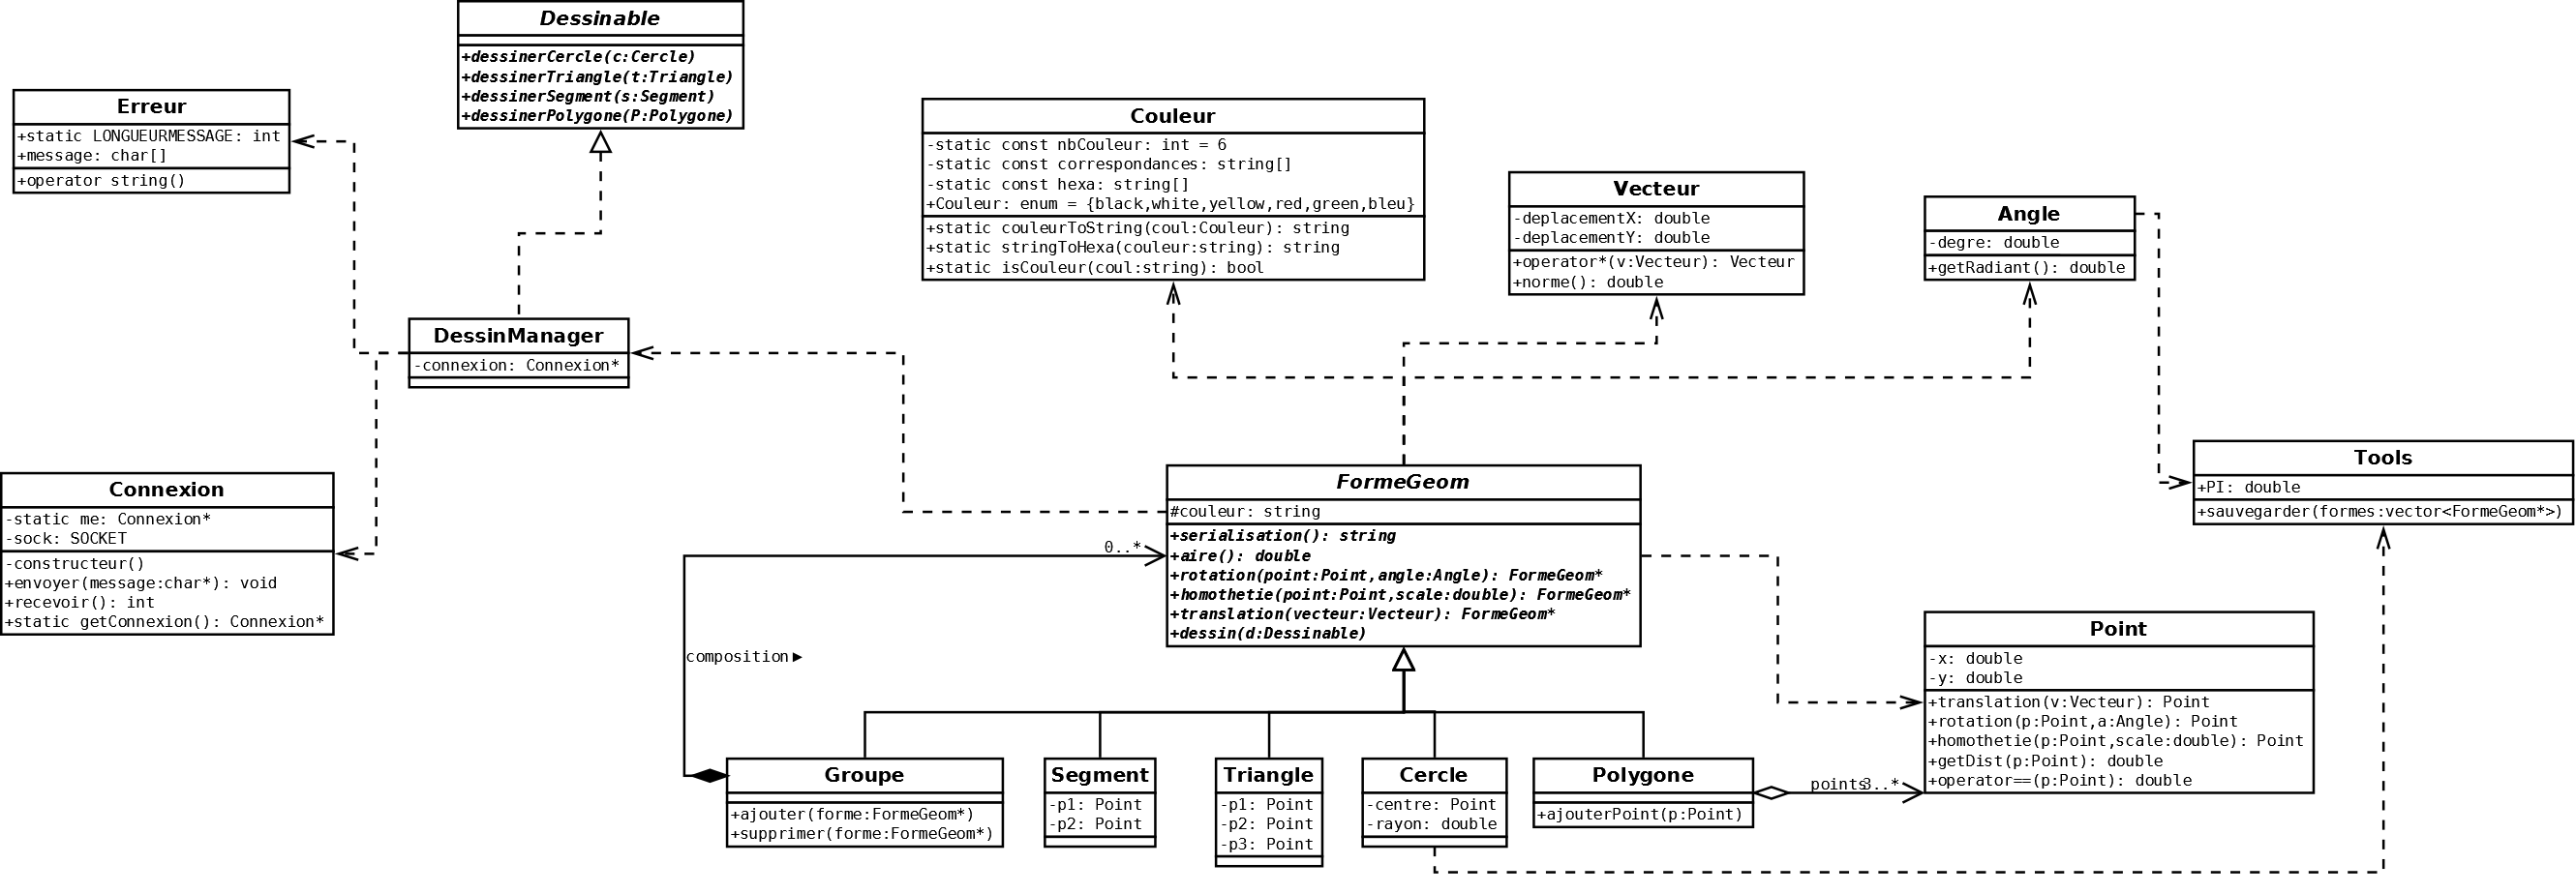
\includegraphics[height=380pt, width=450pt]{DiagrammeDeClasses.png}
\caption{Diagramme de classe de la base du client}
\end{figure}

Encore une fois on peut décomposer cette hiérarchie en plusieurs parties:
\begin{itemize}
\item La partie dessin / connexion au serveur
\item FormeGeom et ses classes filles
\item Les classes outils
\end{itemize}

\section{Dessin / connexion au serveur}
La partie dessin / connexion au serveur est une partie importante du projet, qui a nécessité une attention particulière car elle se doit d'être le plus modulable possible. En effet, la partie dessin, qui utilise une connexion réseau doit pouvoir être remplacée dans le programme principal par une partie dessin quelconque (par exemple une qui utiliserait directement une bibliothèque graphique). C'est pourquoi cette partie respecte le Design Pattern Visitor. 
\subsection{Design Pattern Visitor}
Ce Design Pattern permet d'appeler des méthodes spécifiques à une classe depuis une autre partie du programme tout en gardant le polymorphisme de la classe. Dans ce cas précis cela se traduit par le fait qu'il est possible de lancer la méthode de dessin spécialisée d'une forme sans violer le principe de substitution de Liskov\footnote{principe de substitution de Liskov: "Si $q(x)$ est une propriété démontrable pour tout objet $x$ de type $T$, alors $q(y)$ est vraie pour tout objet $y$ de type $S$ tel que $S$ est un sous-type de $T$". Sources: \url{http://programmers.stackexchange.com/questions/178488/lsp-vs-ocp-liskov-substitution-vs-open-close} et \url{http://fr.wikipedia.org/wiki/Principe_de_substitution_de_Liskov} }, c'est à dire sans implémenter la méthode de dessin directement dans la classe abstrait et d'utiliser une fonction du type \textit{typeid} pour savoir quelle classe particulière l'appelle.
La mise en oeuvre de ce Design Pattern est très simple, il suffit de d'implémenter les méthodes de dessin spécialisées ( dessinerTriangle, dessinerSegment etc.) dans la classe \textit{Dessin}, puis d'appeler la bonne méthode spécialisée dans la méthode générale $dessin$ de chacune des classe, par exemple on pourra avoir:
\begin{figure}[H]
\begin{verbatim}
void Segment::dessin(const Dessin &d) const{
    d.dessinerSegment(*this);
}
\end{verbatim}
\caption{Une implémentation possible de la méthode dessin de la classe segment}
\end{figure}
Et ainsi on pourra appeler la méthode dessin sur un pointeur de \textit{FormeGeom} tout en étant sûr que la bonne méthode spécialisée va être appelée.

\subsection{Interface Dessinable}
Le problème de la solution précédente, c'est que si jamais on veut changer la de dessin, par exemple pour utiliser une bibliothèque graphique C++, on ne peut pas garantir que toutes les méthodes spécialisées dont on a besoin seront présentes. De plus comme cette solution ne permet de dessiner que avec la classe \textit{Dessin}, il faudra réécrire par dessus la classe existante, et on ne pourra pas utiliser deux façons de dessiner différentes dans le même programme (par exemple si on veut d'abord afficher à l'aide d'une bibliothèque C++ puis dessiner sur le serveur). La solution à ce problème est très simple: on crée une classe abstraite qui définira le comportement que doit avoir une classe de dessin ( il s'agit donc d'une interface ) et on définie la méthode \textit{dessin} de \textit{FormeGeom} comme utilisant un objet de implémentant cette classe. Ainsi on est sûr que les classes de dessins devront être correctement implémentées et en plus on peut en utiliser plusieurs différentes dans le même programme.
On obtiendra donc une implémentation finale ressemblant à cela:
\begin{figure}[H]
\begin{verbatim}
void Segment::dessin(const Dessinable &d) const{
    d.dessinerSegment(*this);
}
\end{verbatim}
\caption{L'implémentation de la méthode dessin dans segment en utilisant l'interface Dessinable.}
\end{figure}

\subsection{Connexion}
\subsubsection{principe}
La classe \textit{Dessin} qu'il était demandé d'implémenter devait créer une connexion avec le serveur java. Il a donc été décidé de créer une classe s'occupant de gérer la connexion et d'en faire un composant de la classe \textit{Dessin}.
\subsubsection{la classe}
La classe \textit{Connexion} est plutôt simple à réaliser, en effet elle est simplement composée d'un constructeur dans lequel on passe l'adresse ip et le numéro de port du serveur, d'une méthode d'envoi de données et d'une méthode de réception.
\subsubsection{singleton}
À la conception de cette classe s'ajoute un problème: sous Windows le chargement de la dll winsock2 ne doit se faire qu'une seul fois dans toute la durée de vie du programme. Il faut faire de ce chargement un singleton. Pour ce faire, il suffit de créer une méthode statique qui se chargera uniquement de charger la dll, et d'ajouter une variable de type bool elle aussi statique et initialisée à \textit{false}. Le principe étant que à la création d'une connexion, on vérifie si vaut bien \textit{false}, et si c'est le cas on appelle la méthode de chargement de la dll, qui elle même passera le booléen à \textit{true} afin de ne plus jamais être appelée.

\subsubsection{code multiplateforme}
La bibliothèque winsock2 étant fortement inspirée des sockets unix, il est très facile de rendre le code compilable sous un système unix (incluant linux et mac) simplement avec quelques instructions $define$ et de ne lancer les bouts de code spécifique à une plateforme grâce à des conditions préprocesseur.
Sans entrer dans les détails voici le chargement des bibliothèques nécessaires ainsi que les $define$ qui permettent d'avoir un code multiplateforme:
\begin{figure}[H]
\begin{verbatim}
#ifdef  __unix__

    #include <sys/types.h>
    #include <sys/socket.h>
    #include <netinet/in.h>
    #include <arpa/inet.h>
    #include <unistd.h>
    #include <errno.h>

    #define INVALID_SOCKET -1
    #define SOCKET_ERROR -1
    #define WSAGetLastError() errno
    #define SD_BOTH 2
    #define closesocket(s) close(s)
    typedef int SOCKET;
    typedef struct sockaddr_in SOCKADDR_IN;
    typedef struct sockaddr SOCKADDR;

#else

    #include <winsock2.h>
    #pragma comment(lib, "ws2_32.lib") // spécifique à VISUAL C++
    #if (MSVC++ 12.0 _MSC_VER == 1800)
        #define strdup _strdup
    #endif

#endif
\caption{le chargement des bibliothèques selon le système d'exploitation}
\end{verbatim}
\end{figure}


\subsection{fonctionnement du tout}
On a donc une classe servant à dessiner des formes en les envoyant à un serveur distant. Il faut donc définir un protocole d'envoi, afin que les deux parties (client et serveur) puisse communiquer correctement.
Tout d'abord il y a le format de l'envoie, il a été décidé que chaque forme serait envoyé sous la forme d'une chaîne de caractères grâce à la méthode \textit{toString()}(voir \ref{toString} ) des formes géométriques.
Les formes seront envoyées une par une (dans le cas ou vous envoyez un groupe de forme), afin de faciliter la lecture du côté serveur (pas besoin d'envoyer des informations inutiles comme le groupe de départ, puisque cela ne correspond à rien au niveau de l'affichage).
Pour conclure voici un diagramme de classe représentant cette partie entière:
\begin{figure}
\includegraphics[height=380pt, width=450pt]{connexion.png}
\caption{le diagramme de classe de la partie dessin}
\end{figure}


\section{FormeGeom et ses classes filles}
Cette partie, qui est au cœur du projet est évidemment celle qui a nécessitée le plus d'attention.
\subsection{Premières réflexions}
En partant d'une hiérarchie très simple où chaque objet géométrique (segment, triangle, cercle, polygone et groupe de formes) est représenté par une classe; on définie toutes les opérations et les propriétés voulues pour chacune de ces classes. Une fois cela fait, on compare les classes entre elles et s'il y a des points commun on les remonte dans une classe supérieur. Très vite on remarque donc que tout ces objets partagent plusieurs opérations:
\begin{itemize}
\item les transformations géométriques
\item la possibilité d'être sauvegardé dans un fichier ou chargé depuis une sauvegarde
\item une opération de dessin
\item une opération de transformation en chaine de caractère
\item une opération calculant l'aire de la forme
\end{itemize} 
ainsi que deux propriétés:
\begin{itemize}
\item le groupe auquel la forme appartient (si la forme appartient)
\item la couleur de la forme
\end{itemize}
On rassemble donc toutes ces propriétés dans une classe abstraite dont hériteront tous les objets géométriques. Appelons cette classe FormeGeom, on a donc une première hiérarchie ressemblant à cela:
\begin{figure}[H]
\includegraphics[height=190pt, width=375pt]{premieres_reflexions.png}
\caption{Première ébauche de diagramme de classe}
\end{figure}


\subsection{Les points}
Parmi les zones d'ombre restantes il y a la représentation des coordonnées d'une figure géométrique. Une solution simple et intuitive pour représenter des coordonnées est le point, caractérisé par deux valeurs (pour un point en 2 dimensions) x et y, il sera utilisé en tant que composant de certaines formes géométrique (cercle, segment et triangle). On crée donc la classe associée Point et naïvement on arrive à cette configuration:
\begin{figure}[H]
\includegraphics[width=600pt,height=300pt]{premier_point.png}
\caption{première implémentation de point}
\end{figure}
Cette configuration fut considérée comme suffisamment factorisée et stable (c'est à dire que même si des modifications devaient être apportées, le principe serait préservé) pour commencer à développer le reste du logiciel.


\subsection{pistes abandonnées}
Néanmoins, lors du développement d'autres structures ont été envisagée, ou même temporairement implémentée.
Ainsi il a été envisagé de créer des sous catégories de formes géométriques selon le nombre de points qui les composent, par exemple \textit{cercle} héritera de la classe abstraite \textit{Forme1point}, cette dernière contient le point \textbf{p1} et définitions des transformations géométriques sur \textbf{p1}; et ainsi on pourra avoir une seconde classe \textit{Forme2point} héritant de \textit{Forme1point}, dans le but de ne pas réécrire ni la variable \textbf{p1}, ni les opérations sur celui ci. Cette solution n'a pas été retenue car, en plus de ne pas factoriser énormément de code, elle ajoute de la complexité qui n'est pas forcément pertinente. Par exemple on pourrait très bien définir des formes simple à l'aide d'équation plutôt que de points, et dans ce cas ce modèle ne permet pas de les intégrer simplement à la hiérarchie. Cette solution n'est donc pas suffisamment générique.
%%%%%%%%%%%%%%%%%%%%%%%%%%%% TODO

\subsection{Forme finale}
\subsubsection{Points}
Finalement il s'avère que les transformations géométriques (translation, homothétie et rotation) qui devaient s'appliquer aux formes géométriques simple devaient aussi avoir une implémentation dans \textit{Point}. Cependant, il semblait que la classe \textit{Point} ne pouvait pas hériter de \textit{FormeGeom} car il n'était pas demandé de dessiner \textit{Point}, ni pouvoir le sauver/charger et un point n'a pas de couleur. C'est pourquoi à un moment du développement il a été décidé de créer une classe au dessus de \textit{FormeGeom} pour regrouper les transformations géométriques et la transformation en chaîne de caractères ( utilisée aussi par \textit{Point} ). On est donc arrivé à une architecture proche de celle-ci:
\begin{figure}[H]
\includegraphics[width=400pt,height=300pt]{objet_geom.png}
\end{figure}
\subsubsection{Formes composées}
Enfin on peut remarquer que les classes \textit{Polygone} et \textit{GroupeDeForme} sont très proches, puisque globalement elles effectuent le même travail, c'est à dire appliquer des opérations sur une liste d'objets géométrique. On peut donc factoriser ces opération à l'aide d'une classe abstraite supérieur. Seulement, bien que les les classes \textit{Polygone} et \textit{GroupeDeForme} utilisent des objets dérivant de \textit{ObjetGeom}, \textit{GroupeDeForme} utilise des pointeurs pour bénéficier du polymorphisme sur les classes héritant de \textit{FormeGeom}, alors que \textit{Polygone} utilise directement des \textit{Point}. Si on veut factoriser ces classes il faut choisir un type de variable: variable brut ou pointeur sur la variable, or \textit{GroupeDeForme} est obligé d'utiliser des pointeurs, alors que polygone n'est pas contraint. La classe abstraite au dessus de ces classes manipulera donc un ensemble de pointeurs sur ObjetGeom, cela a le désavantage de rendre l'écriture moins élégante dans les quelques méthodes que \textit{Polygone} devra implémenter, mais le gain en abstraction est suffisant pour compenser.
De plus, la nouvelle classe doit implémenter des méthodes sur un ensemble de données, il  faut donc la doter de cet ensemble de données. On pourrait mettre une variable membre de type vector<ObjetGeom>, mais cela empêcherais d'avoir la précision de quel objet est contenu dans l'ensemble, la solution adoptée est donc d'en faire une classe template que \textit{Polygone} et \textit{GroupeDeForme} implémenteront selon leur besoin.
On a donc une hiérarchie final qui ressemble à ça:
\begin{figure}[H]
\includegraphics[width=400pt,height=300pt]{forme_composee.png}
\end{figure}





\section{Les classes outils}\label{classesOutils}
En plus de ces deux parties nécessaires au bon fonctionnement du programme, un autre type de classe a était utilisé dans ce projet, il s'agit de classes "outil". Il s'agit de classe qui ont pour unique but de faciliter la mise en place le reste de la programmation.
\subsection{classe Vecteur}\label{vecteur}
La classe qui rempli le plus ce rôle est très certainement la classe \textit{Vecteur}, qui comme son nom l'indique représente un vecteur.
Cette classe est utiliser pour faciliter les transformations géométriques. En effet, il est souvent plus facile de procéder (et à lire) à  des opérations sur des vecteur que de les faire de façon naïve. Par exemple:
\begin{figure}[H]
\begin{verbatim}
Point Point::rotation(const Point &p, const double &angle) const{
	double theta = toRadian(angle);
	double x = cos(theta) * (_x - p._x) - sin(theta) * (_y - p._y) + p._x;
	double y = sin(theta) * (_x - p._x) + cos(theta) * (_y - p._y) + p._y;
	return Point(x, y);
}
\end{verbatim}
\caption{fonction de rotation sans vecteur}
\end{figure}
cette fonction permet de calculer un nouveau point suite à une rotation
d'angle \textit{angle} et de rotation \textit{rotation}. Elle fonctionne, pourtant on pourrait encore la rendre plus claire:
\begin{figure}[H]
\begin{verbatim}
Point Point::rotation(const Point &p, const Angle &a) const{
    Vecteur rot(MatriceCarree2::getMatriceRotation(a) * Vecteur(p,*this));
    return   Point(  p._coord + rot );
}
\end{verbatim}
\caption{fonction de rotation avec Vecteur}
\end{figure}
En sachant que \textit{MatriceCarree2::getMatriceRotation(a)} crée la matrice de rotation à partir de l'angle \textit{a} et que \textit{$_coord$} est le vecteur de coordonnées du point p.
On a fait exactement la même choses mais en l'exprimant autrement, et le code s'en trouve plus proche la formule mathématique initiale.
Pour en arriver là, il a fallu recréer quelques opérations sur les vecteurs, telles que le produit scalaire, ou l'addition de vecteur. Ces définitions ont été rendu possible par la surcharge d'opérateurs +, - et *.
Dans l'implémentation du programme, cette classe est totalement encapsulée par la classe \textit{Point}, et n'apparaît en dehors de celle-ci que pour définir une translation.

\subsection{Matrice}
Dans le paragraphe \ref{vecteur} il était question d'utiliser une matrice de rotation pour rendre le code plus élégant.
Une classe représentant les matrices carrées d'ordre 2 à donc été créée pour l'occasion.
Cette classe se veut minimaliste, et ne propose donc qu'une méthode statique de calcule de matrice de rotation, un accesseur statique sur la matrice unité, et la surcharge de l'opérateur* avec un vecteur.
Néanmoins cette classe pourrait très bien être utilisée et améliorée dans le cadre d'une évolution du logiciel.

\subsection{couleurs}\label{couleurs}
Dans le sujet, il est dit que chaque forme géométrique doit avoir une couleur.
Faire un simple \textit{typedef CouleurX valeur;} aurait très bien pu suffire, mais la solution d'une classe gérant une enum de couleurs a été choisies, car elle permet d'ajouter des fonctions liées aux couleurs (conversion en string, en int etc. ) et de les conserver dans un ensemble cohérent (la classe).

\subsection{angle}
De la même façon que pour les couleurs dans le paragraphe \ref{couleurs}, on aurait très bien pu définir un angle simplement par un réel, mais faire une classe - ou au moins un namespace- pour regrouper les notions liées aux angles (conversion en radian ou en degré, valeur de PI etc.) correspondait plus à l'idée d'une application évolutive, car on pourrait très bien imaginer que dans le futur on veille ajouter des fonctionnalités à un angle, il faudra alors de toute manière utiliser une classe et on serait contraint de naviguer dans un ancien code pour trouver à quels endroit il utiliser cette classe.

\subsection{tools.h}
Enfin un fichier sert à regrouper toutes les fonctions qui n'ont pas à être rattachées à une nouvelle classe, il s'agit du fichier tools.h. Il a servit de fichier tampon pendant tout le temps du développement, et maintenant il contient surtout des fonctions liées aux chaines ( split, trim etc. ).

\chapter{L'implémentation du Design Pattern COR}\label{COR}
Cette partie, bien qu'étant une sous partie de la précédente mérite une section séparée.
En effet le Design Pattern COR a une place importante dans ce projet, puisque il est utilisé à la fois du côté serveur pour dessiner les objets reçu et du côté client pour charger les formes sauvegardées. Son fonctionnement et son implémentation étant quasiment identique dans les deux cas, ces deux points seront détaillés une seul fois ici, puisque la version client est la plus aboutie.
\section{Pourquoi faire ?}
Dans les deux utilisation, ce Design Pattern sert avant tout à parser(analyser) le un texte représentant une forme géométrique. Dans le cas du serveur, il s'agit de parser pour pouvoir dessiner par rapport aux données obtenues. Alors que dans le cas du client le parse sert à recréer totalement une forme géométrique. Afin de pouvoir parser correctement, il est judicieux de décomposer la fonction en plusieurs méthodes, chacune spécialisée dans le parse d'un objet en particulier (par exemple on peut imaginer la méthode \textit{parseSegment}, spécialisé dans le parse d'un \textit{Segment}) et de les appeler à la suite. Ces ce principe que le Design Pattern Chain Of Responsibility généralise, en donnant à chaque méthode spécialisée une classe, dite \textit{Experte}, et en permettant à une classe en cas d'échec de sa méthode d'appeler une autre classe \textit{Experte} pour quelle fasse de même. 

\section{Comment ?}
Le principe étant très simple et générique, il a été décidé de créer une classe template afin de ne plus avoir à recréer la hiérarchie du Design Pattern. De plus l'utilisation de ce Design pattern est grandement simplifié lorsqu'on le couple avec le Design Pattern Facade, ayant pour but de regrouper la création de la liste à un seul endroit et de la cacher à l'utilisateur. Par exemple, au lieu de devoir créer une liste d'expert à chaque fois, puis de prendre le premier chaînon et d'appeler la bonne méthode, l'utilisateur n'aura qu'a instancier une facade et à appeler la seul méthode de celle-ci (nommée \textit{run} dans notre cas).
Tout ceci combiné on obtient le diagramme de classe suivant:
\begin{figure}[H]
\includegraphics[width=400pt,height=300pt]{cor.png}
\caption{Le diagramme de classe de la chaîne de responsabilités du client}
\end{figure}
Et la transformation d'un bout de texte en \textit{FormeGeom*} se fait comme ceci dans le programme:
\begin{figure}[H]
\begin{verbatim}
FormeGeom* paserTexte(const string &s){
    return ChargementFacade(s).run();
}
\end{verbatim}
\caption{utilisation de la façade dans le code}
\end{figure}



\chapter{tests unitaires}\label{tests}
\section{Pourquoi faire ?}
Il est important de s'assurer que le code d'un programme soit fiable, et surtout qu'il le reste au cours du temps. C'est précisément à cela que servent les tests unitaires, et c'est donc pour ça qu'il a été décidé d'en intégrer au projet. Ils se sont avérés particulièrement utile car le projet a subit de nombreux changements d'architecture, et à chaque fois les tests unitaire ont pu décrire précisément ce qui ne fonctionnait plus dans le programme.
\section{Comment ?}
La solution donnée dans le cours sur comment effectuer des tests unitaire ne permettant pas concevoir des fichiers de tests suffisamment clairs, il a été décidé que le projet intégrerait son propre framework de test unitaire, relativement pauvre en fonctionnalités, mais suffisant pour effectuer de simples tests de manière lisible et évolutive.
Cette partie du projet peut être décrite par le diagramme de classe suivant:
\begin{figure}[H]
\includegraphics[width=350pt,height=300pt]{tests_unitaires.png}
\caption{diagramme de classe des tests unitaires}
\end{figure}
À l'aide de conventions de nommage et des macros préprocesseur on peut définir une classe de test comme ceci:
\begin{figure}[H]
\begin{verbatim}
#include "../src/angle.h"

CPPTEST(TestAngle)

    Angle droit(180);

    TESTCASE(getRadian,{
         equals(round(droit.getRadian()*100)/100, round(Angle::PI*100)/100);
     });

ENDTEST

\end{verbatim}
\caption{une classe de tests unitaires fonctionnelle}
\end{figure}
Et on défini une façade comme ça:
\begin{figure}[H]
\begin{verbatim}
TESTLAUNCHER(TestLauncher1)

    addTest(new TestAngle());

ENDLAUNCHER
\end{verbatim}
\caption{la façade associé}
\end{figure}
Puis on s'en sert de cette manière dans le code:
\begin{figure}[H]
\begin{verbatim}

\end{verbatim}
\caption{Utilisation de la façade de tests unitaires}
\end{figure}
Qui affiche un résultat formaté comme celui ci:
\begin{figure}[H]
\includegraphics[width=350pt,height=300pt]{resultat_tests_unitaires.png}
\caption{affichage du résultat des tests unitaires}
\end{figure}

\chapter{Diagramme final}
On peut maintenant résumer l'application client par un seul diagramme de classe:

\begin{figure}[H]
\includegraphics[width=650pt,height=400pt,angle=-90]{diagramme_final.png}
\caption{diagramme de classe final}
\end{figure}

\part{Serveur}
\chapter{Architecture}
Ce programme interagissant avec un client en temps réel, il a été décidé de suivre l'architecture MVC, ou Model View Controller, qui permet de séparer le code des classes métiers(Model) de celui des classes graphiques(View) et en gérant les interactions entre les deux avec une classe arbitre (Controller).
Les interactions entre la vue est le contrôleur sont définies par des interfaces implémentés par les vues décrivant les opérations que les contrôleurs peuvent effectuer sur  celles-ci (par exemple mettre à jour le nombre de connectés).
À partir de ce point on peut décomposer le programme java en 2 parties:
\begin{itemize}
\item La partie gérant le serveur principal
\item La partie gérant le thread dédié
\end{itemize}
\chapter{partie gérant le thread principal}
Elle est composée de:
\begin{itemize}
\item la classe métier \textit{Server}, qui représente le serveur principal qui tourne en boucle
\item de la vue \textit{ServerStatus} qui affiche l'adresse ip, le port du serveur et le nombre de clients connectés
\item et la classe \textit{ServerStatusCtrl} qui se charge de mettre à jours ces données dans la vue en fonction de \textit{Server}.
\end{itemize} 

\chapter{La partie gérant le thread dédié}
Elle est composée de:
\begin{itemize}
\item la classe métier \textit{DedicatedThread}, qui représente le un thread dédié au client, qui écoute les messages que ce dernier envoie
\item de la vue \textit{DrawingArea} qui affiche les formes en utilisant l'active rendering\footnote{l'active rendering: permet de reprendre le contrôle sur la manière dont est affichée une fenêtre par java en écrivant nous même dessus (par l'intermédiaire de buffers) et en décidant à quel moment afficher les changements.} elle implémente des méthodes de dessin: $drawEllipse$ pour dessiner un cercle, $drawLine$ pour dessiner des lignes, $drawPolygon$ pour les polygones et $showShapes$ pour afficher le buffer sur lequel on travaillait.
\item et la classe \textit{DrawinAreaCtrl} qui se charge de dessiner toutes les formes envoyées par \textit{DedicatedThread} via une chaîne de responsabilité très semblable à celle de la partie \ref{COR}.
\end{itemize}
\chapter{La fenêtre de dessin}
Lorsqu'on programme une application graphique, la plupart du temps le point de coordonnée $(0,0)$ se situe en haut à gauche de l'écran et l'axe des $x$ va vers le bas de l'écran, à l'inverse des plan sur lesquels on a l'habitude de travailler en mathématiques. Pour que les coordonnées que l'utilisateur du client a entrées soient représentées comme sur on pourrait l'attendre, il faut donc effectuer des transformation sur le plan. C'est pourquoi le code de la fenêtre de dessin contient une méthode qui effectue ces transformations et place les nouveaux axes x et y obtenu.
On obtient donc quelque chose comme ça:
\begin{figure}[H]
\includegraphics[width=300pt, height=200pt]{axes.png}
\caption{La fenêtre de dessin}
\end{figure}

\newpage




\part{Fonctionnement de l'application distribuée}
\chapter{Fonctionnement général}
L'application distribuée fonctionne de cette façon: 
Un serveur tourne en continu en écoutant un port donnée.
Côté client on peut créer des formes géométriques et effectuer des transformations dessus.
Quand le l'utilisateur du client a envie de dessiner une forme pour la première fois, une demande de connexion est envoyé au serveur.
Quand le serveur reçoit la demande de connexion, il ouvre un nouveau Thread chargé de dialoguer avec le client ainsi qu'une fenêtre dédiée, et acquitte la connexion.
Le client reçoit l'acquittement et envoie l'objet géométrique sous forme de chaîne au Thread dédié.
Le Thread réceptionne la chaîne de caractères et acquitte le message.
Ensuite il traite la chaîne et l'affiche dans la fenêtre grâce au Design Pattern COR (voir \ref{COR}).
Résumé du fonctionnement:
\begin{figure}[H]
\includegraphics[width=300pt,height=300pt]{fonctionnement_client_serveur.png}
\caption{diagramme de séquence du fonctionnement de l'application distribuée}
\end{figure}


%%%%%%%%%% protocole de com	 => xml et json == overkill + human readability not required

\part{Organisation du projet}

\chapter{méthodes}

Afin d'organiser correctement le projet, il a été décidé qu'il serait réalisé en suivant des méthodes agiles (sans les suivre strictement) et plus particulièrement le tableau Srum a joué un rôle central dans ce projet. Il s'agit d'un tableau dans lequel on place les tâches et sous tâches à réaliser et leur état d'avancement ( à faire, en cours, fini), ce tableau a pour but de stimuler l'avancement et de mieux connaître ses capacités (on remarque que tel type de tâche peuvent être réalisées en tant de temps, que tel autre est plus difficile etc. ). Un autre points des méthodes agiles qui a eu un rôle de premier ordre est: les tests unitaire, leur fonctionnement est détaillé en \ref{tests}.
\chapter{Outils utilisés}
Pour mener à bien ce projets, plusieurs outils autres qu'un IDE ont été utilisés:
\begin{itemize}
\item Trello, un site internet qui permet de créer et d'organiser des listes d'y assigner des utilisateur et d'autres choses en rapport avec l'organisation d'un projet. Il a été utilisé pour mettre en place le tableau scrum et archiver les question et réponses en rapport avec le sujet. Un visuel du site:
\begin{figure}[H]
\includegraphics[width=300pt,height=300pt]{trello.png}
\caption{une capture d'écran du tableau scrum sur le site Trello}
\end{figure}
\item Github, qui est une interface à l'outil de gestion de fichiers git et sur lequel le projet est hébergé.
\end{itemize} 

\part{Conclusion}
Ce projet m'a permit d'augmenter mes connaissances dans des notions de programmation orienté objet avancées telles que les template, et les spécificités de C++11 comme les fonctions lambda ou les conteneurs et les fonctions associées (foreach, find ...). Mais il m'a aussi fait découvrir des nouvelles notions, comme les Design Pattern Visitor et COR ou l'active rendering. Et enfin je pense avoir acquis de nouvelles compétences, notamment en organisation.



\end{spacing}
\end{document}